
Raft is a consensus algorithm for replicated logs which correspond to
replicated the state machine (all servers execute same commands in same order).

\begin{center}
    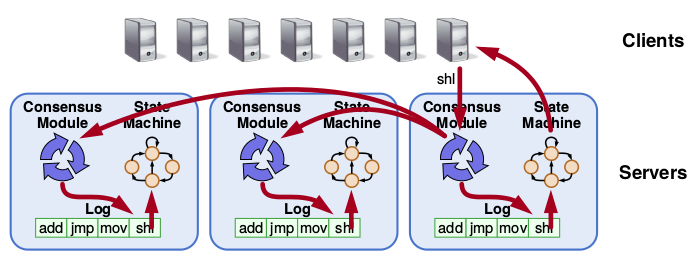
\includegraphics[width=9cm]{img/raft}
\end{center}

\subsection{Client protocol}
Client send command to leader (or other server that will redirect
to leader) and the leader does not respond until command as been
(1) logged, (2) committed and (3) executed by leader's state machine.

\paragraph{Unique ID} has use to identify a client command and has store in
log. This allow to not execute a command twice if leader crashes after
executing command, but before responding.

\subsection{Overview}

\subsubsection{Consensus}
Consensus is leader-based which is more efficient thant leader-less approach
and allow to simplifies normal operation because there is no conflict.

\subsubsection{Server states}

\begin{itemize}
    \item At any given time, each servier is EITHER :
        \begin{enumerate}
            \item Follower : completely passive 
            \item Candidate : used to elect a new leader
            \item Leader: handles all client interactions, log replication
        \end{enumerate}
    \item Time divided into term (maintains current term value)
\end{itemize}

\begin{center}
    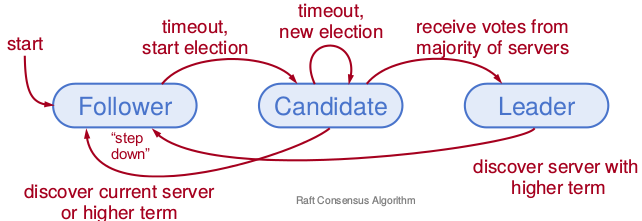
\includegraphics[width=9cm]{img/rleader}
\end{center}

\subsubsection{Terms}
\begin{tabular}{m{8cm}m{6cm}}
    Time divided into term
    \begin{itemize}
        \item at most one leader per term
        \item If no leader on term then failed election
    \end{itemize}
    Term is used to identify obsolete information
    &
    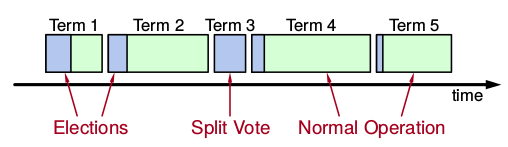
\includegraphics[width=9cm]{img/term}
\end{tabular}

As every RPC contain term of send, \textbf{terms} are used to detect stale
leaders (and candidates) because each election increment the term counter.
\begin{itemize}
    \item If sender’s term is older, RPC is rejected, sender reverts to
        follower and updates its term
    \item if receiver’s term is older, it reverts to follower, updates its term,
        then processes RPC normally
\end{itemize}

\subsubsection{Heartbeats}
\begin{itemize}
    \item Servers start up as followers
    \item Followers expect to receive RPCs from leader or candidates
    \item Leader must send heartbeats (empty
        AppendEntries RPCs) to maintain authority.

        \texttt{ElectionTimeout} without receive RPCs $\rightarrow$ assume that
        leader has crashed.
\end{itemize}


\subsubsection{Leader election}

\begin{enumerate}
    \item Increment current term
    \item Change to candidate state
    \item Vote for self
    \item Send \texttt{Request Vote RPC} (which include
        index and term of last log entry) to all other server
        \begin{itemize}
            \item Receive vote from majority $\Rightarrow$ leader
            \item Receive RPC from valid leader $\Rightarrow$ follower state
            \item Election timeout elapse $\Rightarrow$ new election
        \end{itemize}
\end{enumerate}

Note that the candidate is choose in order to have the leader
with the most complete log.

\begin{itemize}
    \item \textbf{Safety}: allow at most one winner per term because
        each server gives only one vote per term and it's impossible two
        have two different candidates with majorities of vote.

    \item \textbf{Liveness}: some candidate must eventually win.

        $T \leq$ Election timeouts $\leq 2T$, so usually one server
        timeout and wins elections before other wake up.
        (Work well if $T >>$ broadcast time)
\end{itemize}

\subsubsection{Normal operation}
\begin{enumerate}
    \item Client sends command to leader
    \item Leader appends command to its log
    \item Leader sends AppendEntries RPCs to followers
    \item Once new entry committed:
        \begin{enumerate}
            \item  Leader passes command to its state machine, returns result to
                client
            \item  Leader notifies followers of committed entries in subsequent
                AppendEntries RPCs
            \item  Followers pass committed commands to their state machines
        \end{enumerate}
\end{enumerate}

If there is crashed/slow followers,
Leader retries RPCs until they succeed.

$\rightarrow$  Performance is optimal if one successful RPC to any majority of
servers.

\subsection{Log}

\subsubsection{Structure}

\begin{tabular}{m{6cm}m{8cm}}
    Leader take commands from clients and replicates its log to other server.
    \begin{itemize}
        \item Entry \textbf{committed} if know to be stored on majority of servers
    \end{itemize}
    Term is used to identify obsolete information
    &
    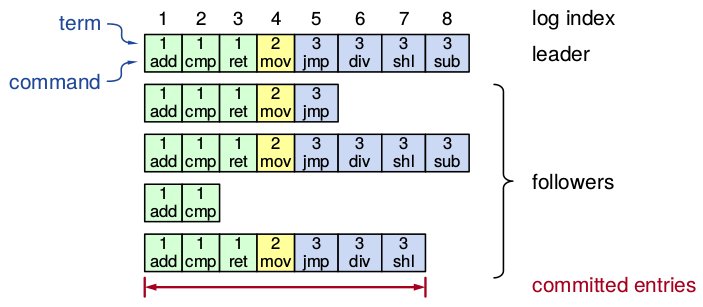
\includegraphics[width=11cm]{img/raftLog}
\end{tabular}

\subsubsection{Consistency}
\begin{itemize}
    \item If log entries on different servers have same index
        and term then (1) they store the same command and (2) the logs are identical
        in all preceding entries
    \item If a given entry is committed, all preceding entries are also committed
\end{itemize}

\subsubsection{Safety}
Raft safety property say that if a leader has decided that a log entry is committed, that entry
will be present in the logs of all future leaders.

To guarantee the safety requirement:
\begin{itemize}
    \item Leaders never overwrite entries in their logs
    \item Only entries in the leader’s log can be committed
    \item Entries must be committed before applying to state machine
\end{itemize}

\subsubsection{Append entries}
Each \texttt{AppendEntries RPC} contains index and term of entry preceding new
ones. This entry must match before append the new entry.

\subsubsection{Commitment rules}
If a leader decide to commit an entry:
\begin{enumerate}
    \item this entry must be stored on a majority of server
    \item \textbf{AND} at least one new entry from leader's term must 
        also be stored on majority of servers
\end{enumerate}

\begin{center}
\begin{tabular}{m{7cm}cm{7cm}}
    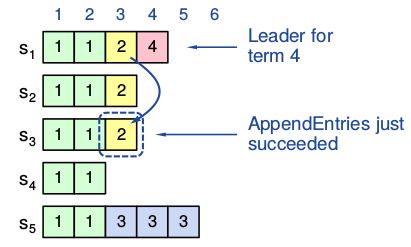
\includegraphics[width=7cm]{img/commitFault}
    &
    $\Rightarrow$
    &
    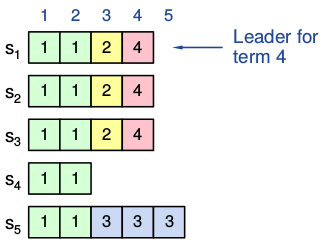
\includegraphics[width=6cm]{img/commitRight}
    \\
    Not safe commit for previous term because $s_5$ can
    be the next leader. (Without 2. commitment rules)
    & &
    Safe commit because $s_5$ cannot be the next leader
    (With 2. commitment rules) \\
\end{tabular}
\end{center}


\subsubsection{Repairing follower logs}
Leader must make follower logs consistent with its own
by (1) delete extraneous entries and (2) fill in missing entries.

\begin{tabular}{m{6cm}m{8cm}}
    \begin{itemize}
        \item Leader keep \textbf{nextIndex} for each follower (initialized
            to $1+leaderIndex$)
        \item When AppendEntries consistency check fails, decrement
            nextIndex and try again
        \item Not that when follower overwrites inconsistent entry, it
            deletes all next entries
    \end{itemize}
    &
    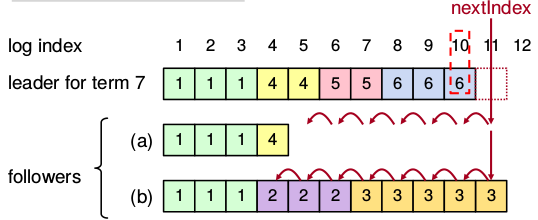
\includegraphics[width=11cm]{img/repairing}
\end{tabular}

\subsection{Configuration}
%TODO slide 27-28-29-30 for 12


